%!TEX root = ../template.tex
%%%%%%%%%%%%%%%%%%%%%%%%%%%%%%%%%%%%%%%%%%%%%%%%%%%%%%%%%%%%%%%%%%%
%% chapter1.tex
%% NOVA thesis document file
%%
%% Chapter with introduction
%%%%%%%%%%%%%%%%%%%%%%%%%%%%%%%%%%%%%%%%%%%%%%%%%%%%%%%%%%%%%%%%%%%

\typeout{NT FILE chapter2.tex}%

\chapter{Background}
\label{cha:Background}

\prependtographicspath{{Chapters/Figures/Covers/}}

\section{Software Quality}

Quality characteristics are specific properties of software, such as correctness, robustness, readability, and evolvability, which can be measured. The primary difficulty in improving software quality is not the applicability of a series of good practices but the very foundation that changes with the incorporation of quality from the inception itself in development rather than just depending on testing at the end of development.

\subsection{Understanding Dimensions of Software Quality}

Software quality is multi-dimensional and predominantly project-specific, based on individual needs and contexts. The diverse dimensions include:

\begin{enumerate}
    \item \textbf{Correctness:} This refers to the software performing its intended job accurately without errors.

    \item \textbf{Robustness:} The software's quality for acting many unintended occurrences without failing. Readability: Code that is easily readable by new developers, which improves maintainability.

    \item \textbf{Evolvability:} The ease with which software can be changed to accommodate new requirements or environments.
\end{enumerate}

Each dimension contributes its unique qualities to the overall software, leading to its long-term success and reliability.

\subsection{Maintenance: The Solution, Not a Problem}

Glass challenges the traditional view that software maintenance is a problem to be minimized. He thinks it should be treated as a positive part of the software lifecycle.

The inherent software flexibility and the nature of maintenance activities: Glass assumes that maintenance is related to enhancements and new functionality added, rather than just error fixing, which is only a small part of maintenance efforts. This represents the adaptive and evolutionary nature of software, such that maintenance activities are put in place to ensure continuous improvement and software refinement based on users' changing needs and technology advances. Integrating Quality into Development Quality software development must be incorporated into the software development life cycle to safeguard against issues after deployment, and ensure maintenance costs are not inflated. Testing software continuously from its early initialization is a sure way of capturing a defect at such an early stage. It can be fixed without more cost and effort that would result in later fixing. Adopt practices for quality improvement during development through reviews, continuous integration, etc.



\cite{ManagingMaintenance1983}
 \cite{MaintenanceGlass1998}
    \cite{lientz1980software}
    \cite{MetricsMaintainability1994}
    \cite{osterweil1996strategic}

    
\subsection{Lehman’s Laws of Software Evolution}

Lehman’s Laws of Software Evolution provide insights into the behavior and progression of software over time. Meir M. Lehman and Les Belady formulated these laws based on extensive analysis of industrial engineering projects.

Continual Change: E-type programs, which are systems embedded in the real world, must continuously adapt to remain functional and satisfactory due to changes in their operational environment. This necessity arises from the natural mismatch between the software's state and its evolving context, not from errors or shortcuts by the engineering team \cite{Lehman1996Laws}. This constant adaptation is driven by the need for feedback and changes in the software's environment, making E-type software similar to biological organisms that must evolve to cope with environmental pressures \cite{LehmanLaws1980}.

Increasing Complexity: Over time, software systems inherently become more complex unless continuous efforts are made to control and reduce this complexity. This phenomenon is akin to the second law of thermodynamics, where entropy in a closed system continuously increases. As software evolves to meet new requirements or fix bugs, interaction points within the system increase, adding to its complexity. If unmanaged, this growing complexity makes maintenance and further development increasingly difficult. Balancing the introduction of new features with complexity management is crucial, though resources for both are limited. Consequently, the rate of growth of a system typically slows as it ages \cite{Lehman1978ProgramsCS}.

\section{Identity Governance and Administration}

Identity Governance and Administration (IGA) is crucial in IT operations for managing user identities and access. IGA combines Identity Governance, which focuses on visibility, role management, and attestation, with Identity Administration, which manages user accounts, credentials, and provisioning. IGA ensures secure IT operations, reduces unauthorized access risks, and automates processes for efficiency and compliance.

The primary purpose of IGA is to create a secure IT environment by managing and controlling user access, enhancing data integrity and confidentiality, and preventing misuse. IGA also improves operational efficiency through automation and compliance with regulations.

Key components of IGA include Identity Lifecycle Management, which handles access rights throughout a user's lifecycle, Access Governance, which enforces access policies, Access Administration, which manages access requests and reviews, and Role-Based Access Control, which assigns roles based on job responsibilities. Policy Enforcement and Compliance ensure adherence to security regulations.

Implementing IGA poses challenges like complexity, integration with existing systems, scalability to accommodate growth, and maintaining a balance between security measures and user experience. Effective IGA implementation requires careful planning to address these challenges.


\section{Netwrix Usercube}


How is usercube configuration code related to object oriented code?

Netwrix Usercube is a product that is now part of Netwrix. It is a comprehensive identity and access management solution. Netwrix Usercube enables organizations of all sizes to enhance their security and compliance posture by ensuring that access permissions are granted only to those who need them. It can automate onboarding and offboarding processes, easing the compliance burden.  

The application is better described dividing it in two modules that work together: Identity and Entitlement Management:

\subsection{Identity Management}

A company deals with various identities, including employees and external workers like contractors, who are usually only tracked for billing. It also involves bots and software. All identities requiring work-related entitlements must be represented.

Typically, companies use a separate system for each identity type. Usercube consolidates information from multiple source systems to create a central repository that manages all identities throughout their lifecycle.

Usercube's repository serves as a mediator between data-providing systems, such as HR systems, and data-receiving systems, like Active Directory. This simplifies the connections between systems.

Without an intermediary, adding a new system to n systems requires n sets of rules, resulting in quadratic complexity. With the central repository, adding a new system needs only one additional set of rules, making the complexity linear \cite{UsercubeDocument}.

\begin{figure}[htbp]
  \centering
  \begin{minipage}{0.48\textwidth}
    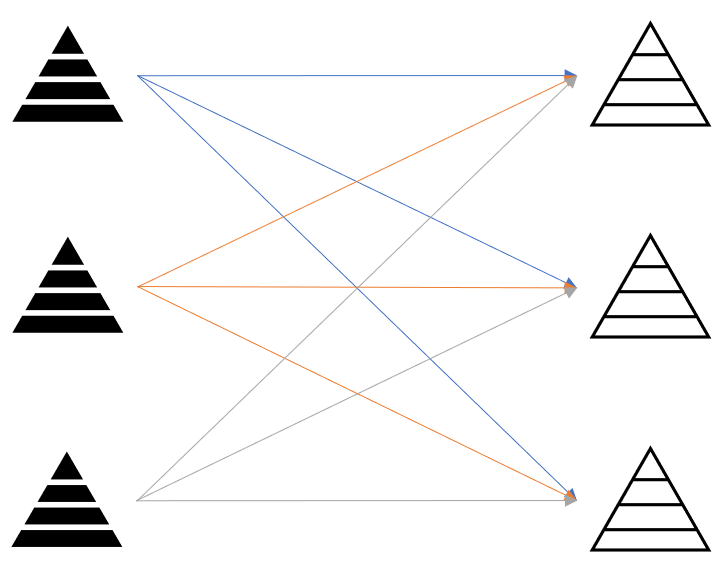
\includegraphics[width=\linewidth]{Identities_complexityQuadratic}
    \caption{Quadratic Complexity}
    \label{fig:Identities_complexityQuadratic}
  \end{minipage}\hfill
  \begin{minipage}{0.48\textwidth}
    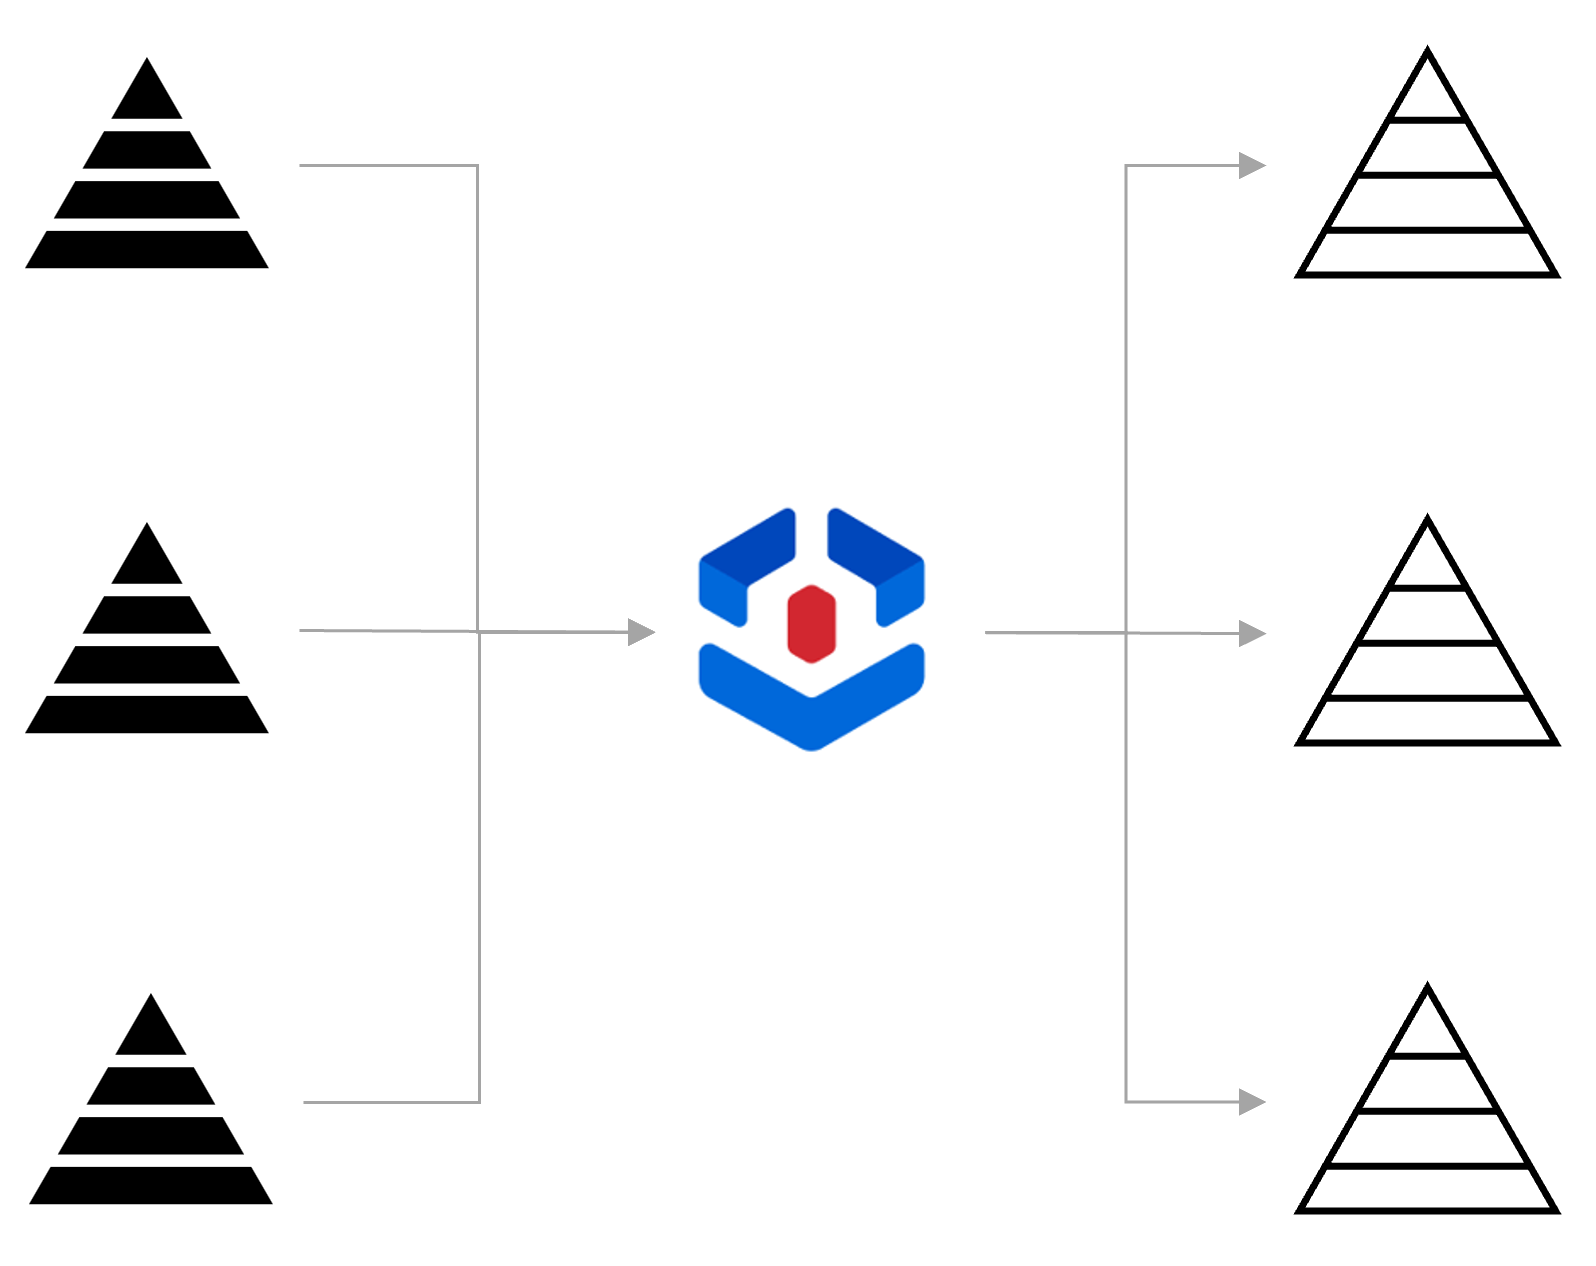
\includegraphics[width=\linewidth]{Identities_complexityLinear}
    \caption{Linear Complexity}
    \label{fig:Identities_complexityLinear}
  \end{minipage}
\end{figure}


\subsection{Entitlement Management}

Entitlement Management involves assigning entitlements to identities, which are permissions allowing access to specific data or locations. In systems like Active Directory, entitlements often manifest as group memberships. Usercube is a tool designed to manage these entitlements by creating a comprehensive catalog and ensuring correct assignments based on a role model that includes governance data and risk definitions.

In Usercube, entitlements are represented as roles within a role catalog that lists all entitlements from managed systems. These roles are linked to specific provisioning rules that write the actual entitlements to the systems, automating the assignment process. For example, to assign an Active Directory entitlement, a rule might add a user to a particular group when a role is assigned. Assignment rules in Usercube automatically assign roles to users based on criteria like job title and location, ensuring compliance and marking unsupported assignments as non-conforming.

Usercube manages different resources through categorized rules, distinguishing between resource types such as standard and administration accounts. This categorization allows for differentiated management, such as setting distinct email addresses and approval workflows for privileged accounts, enhancing security.

\begin{figure}[htbp]
  \centering
  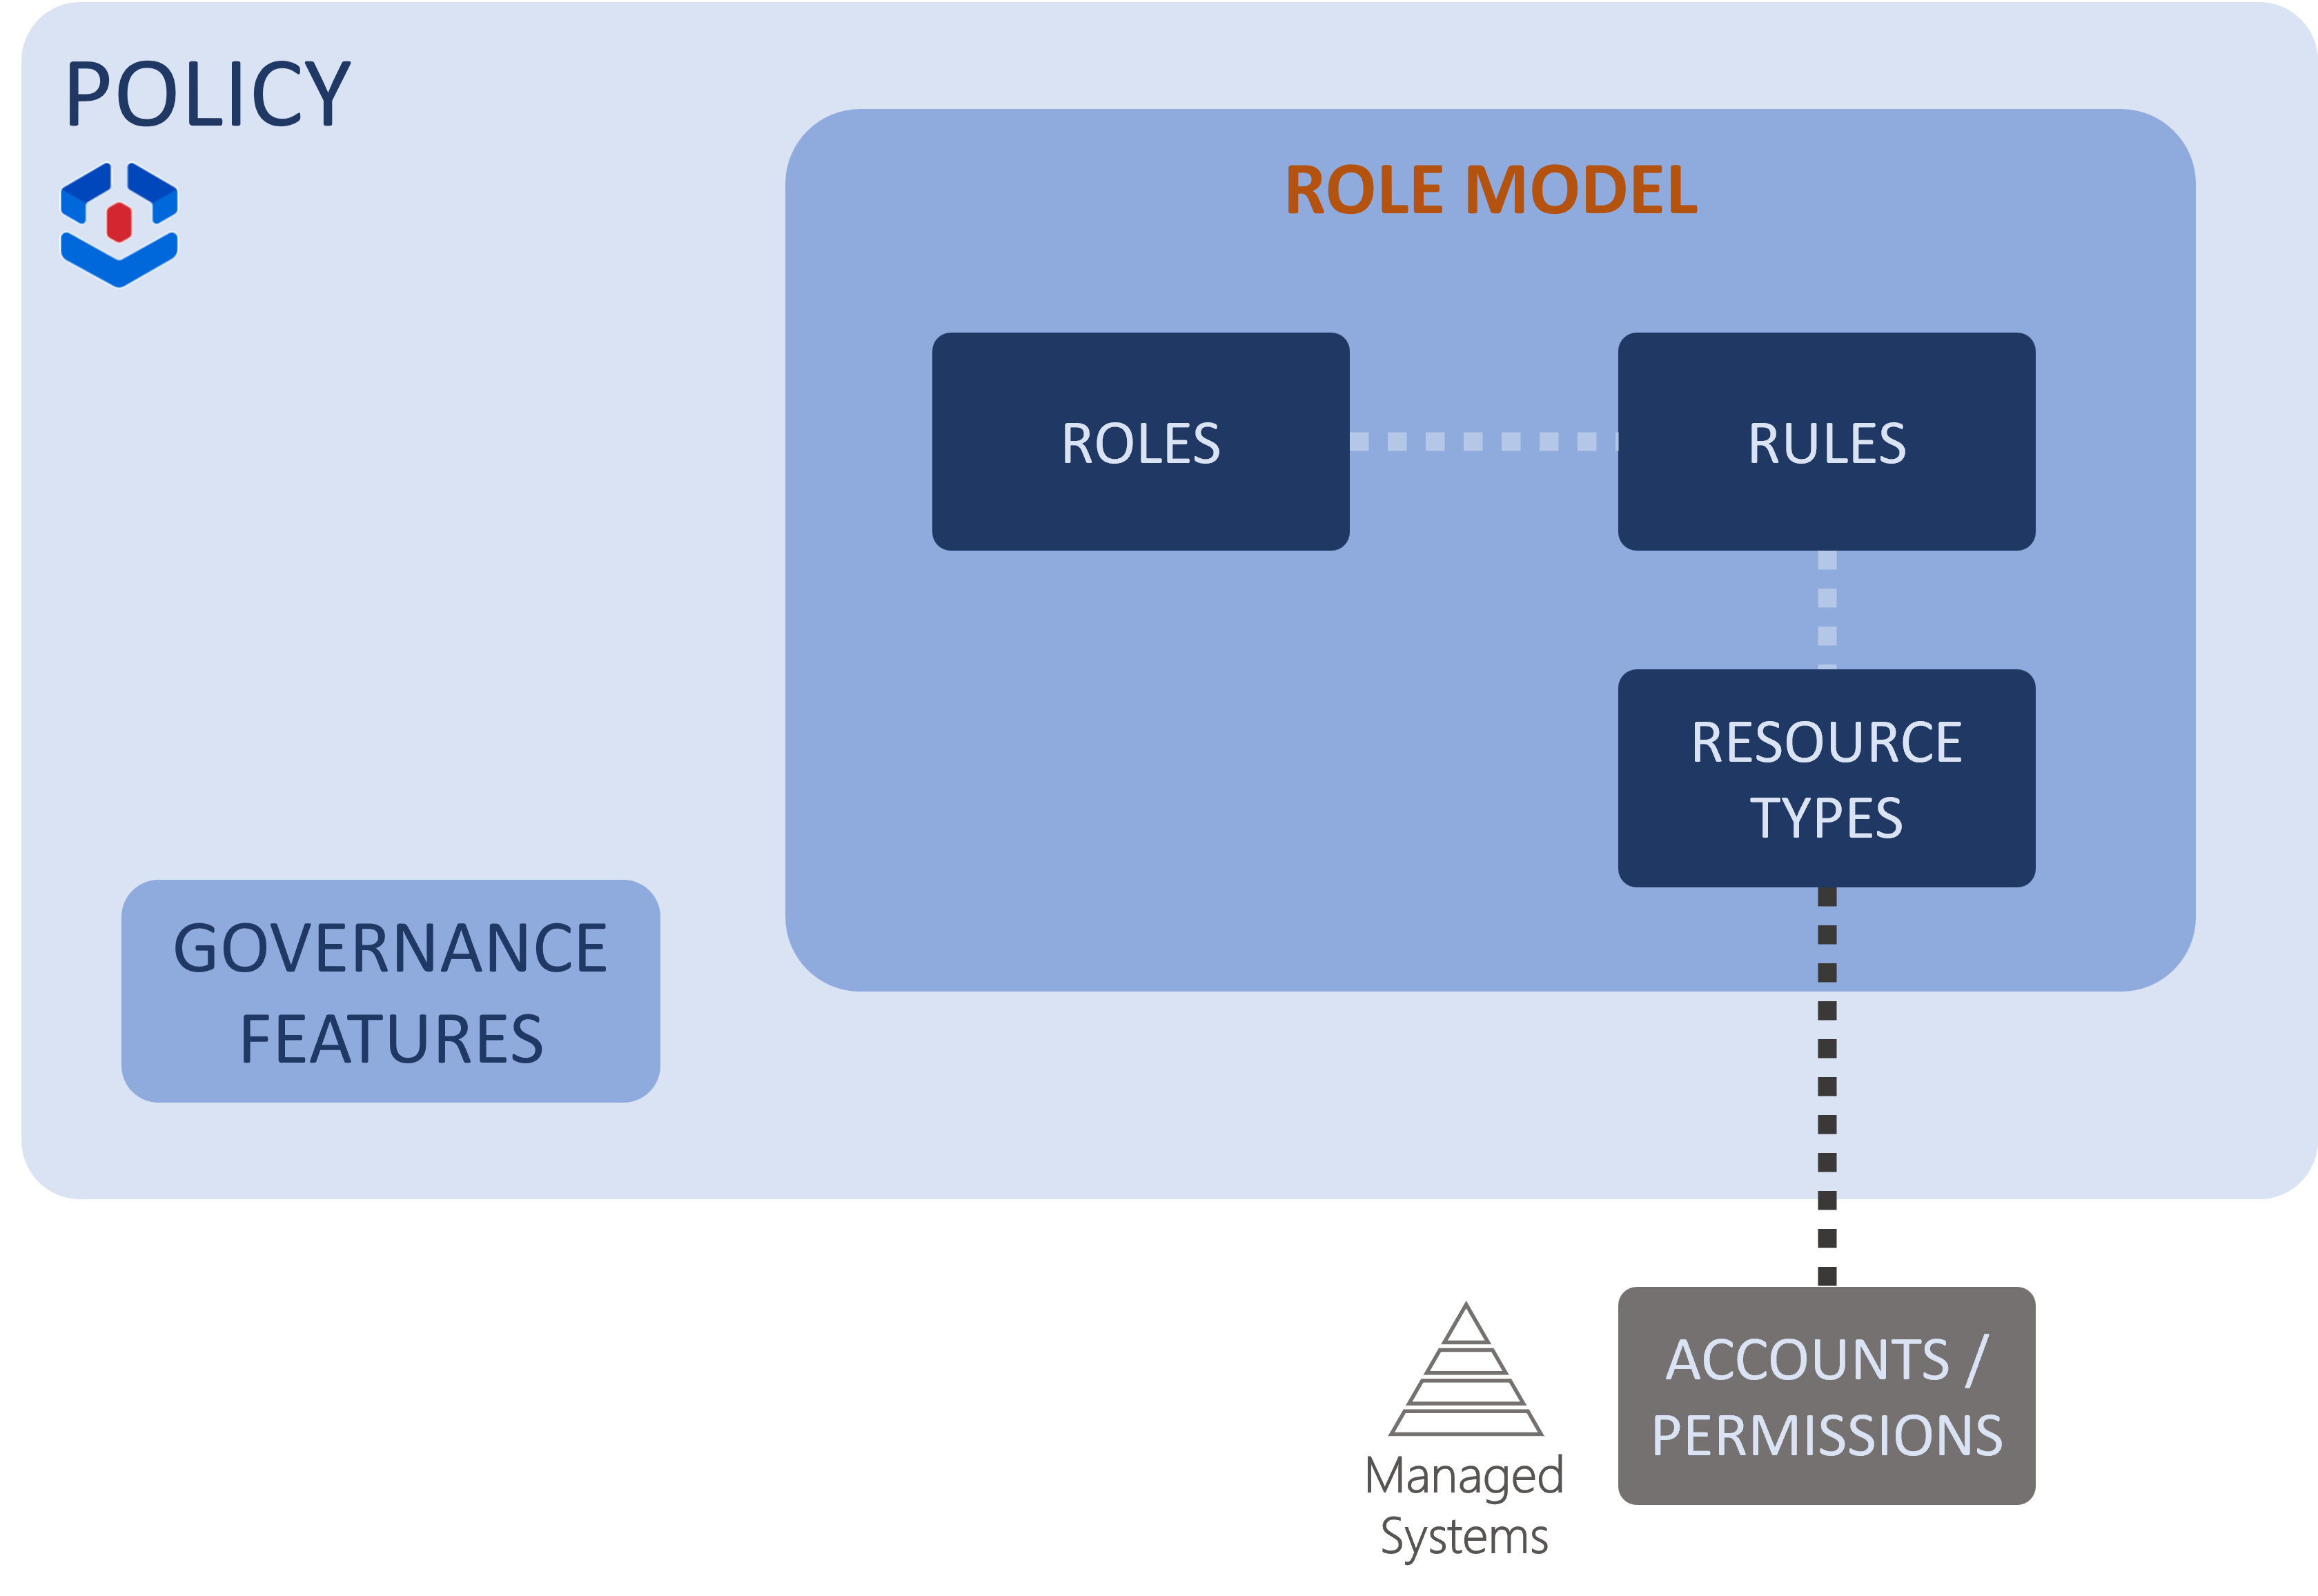
\includegraphics[width=5in]{Entitlements_RoleModel}
  \caption{Entitlements Role Model}
  \label{fig:Entitlements_RoleModel}
\end{figure}

\subsection{Architecture}

Usercube works via a server which operates computation, stores all application data in the database, and serves a web User Interface; at least one agent which operates data flows to/from the managed systems. The managed systems' credentials are used only by the agent and are never disclosed to the server. The agent can call the server, but the server cannot call the agent. The data flows' initiatives are always from the agent. In our case the installation is on-premises so that the server is installed on an isolated network within the company.

\begin{figure}[htbp]
  \centering
  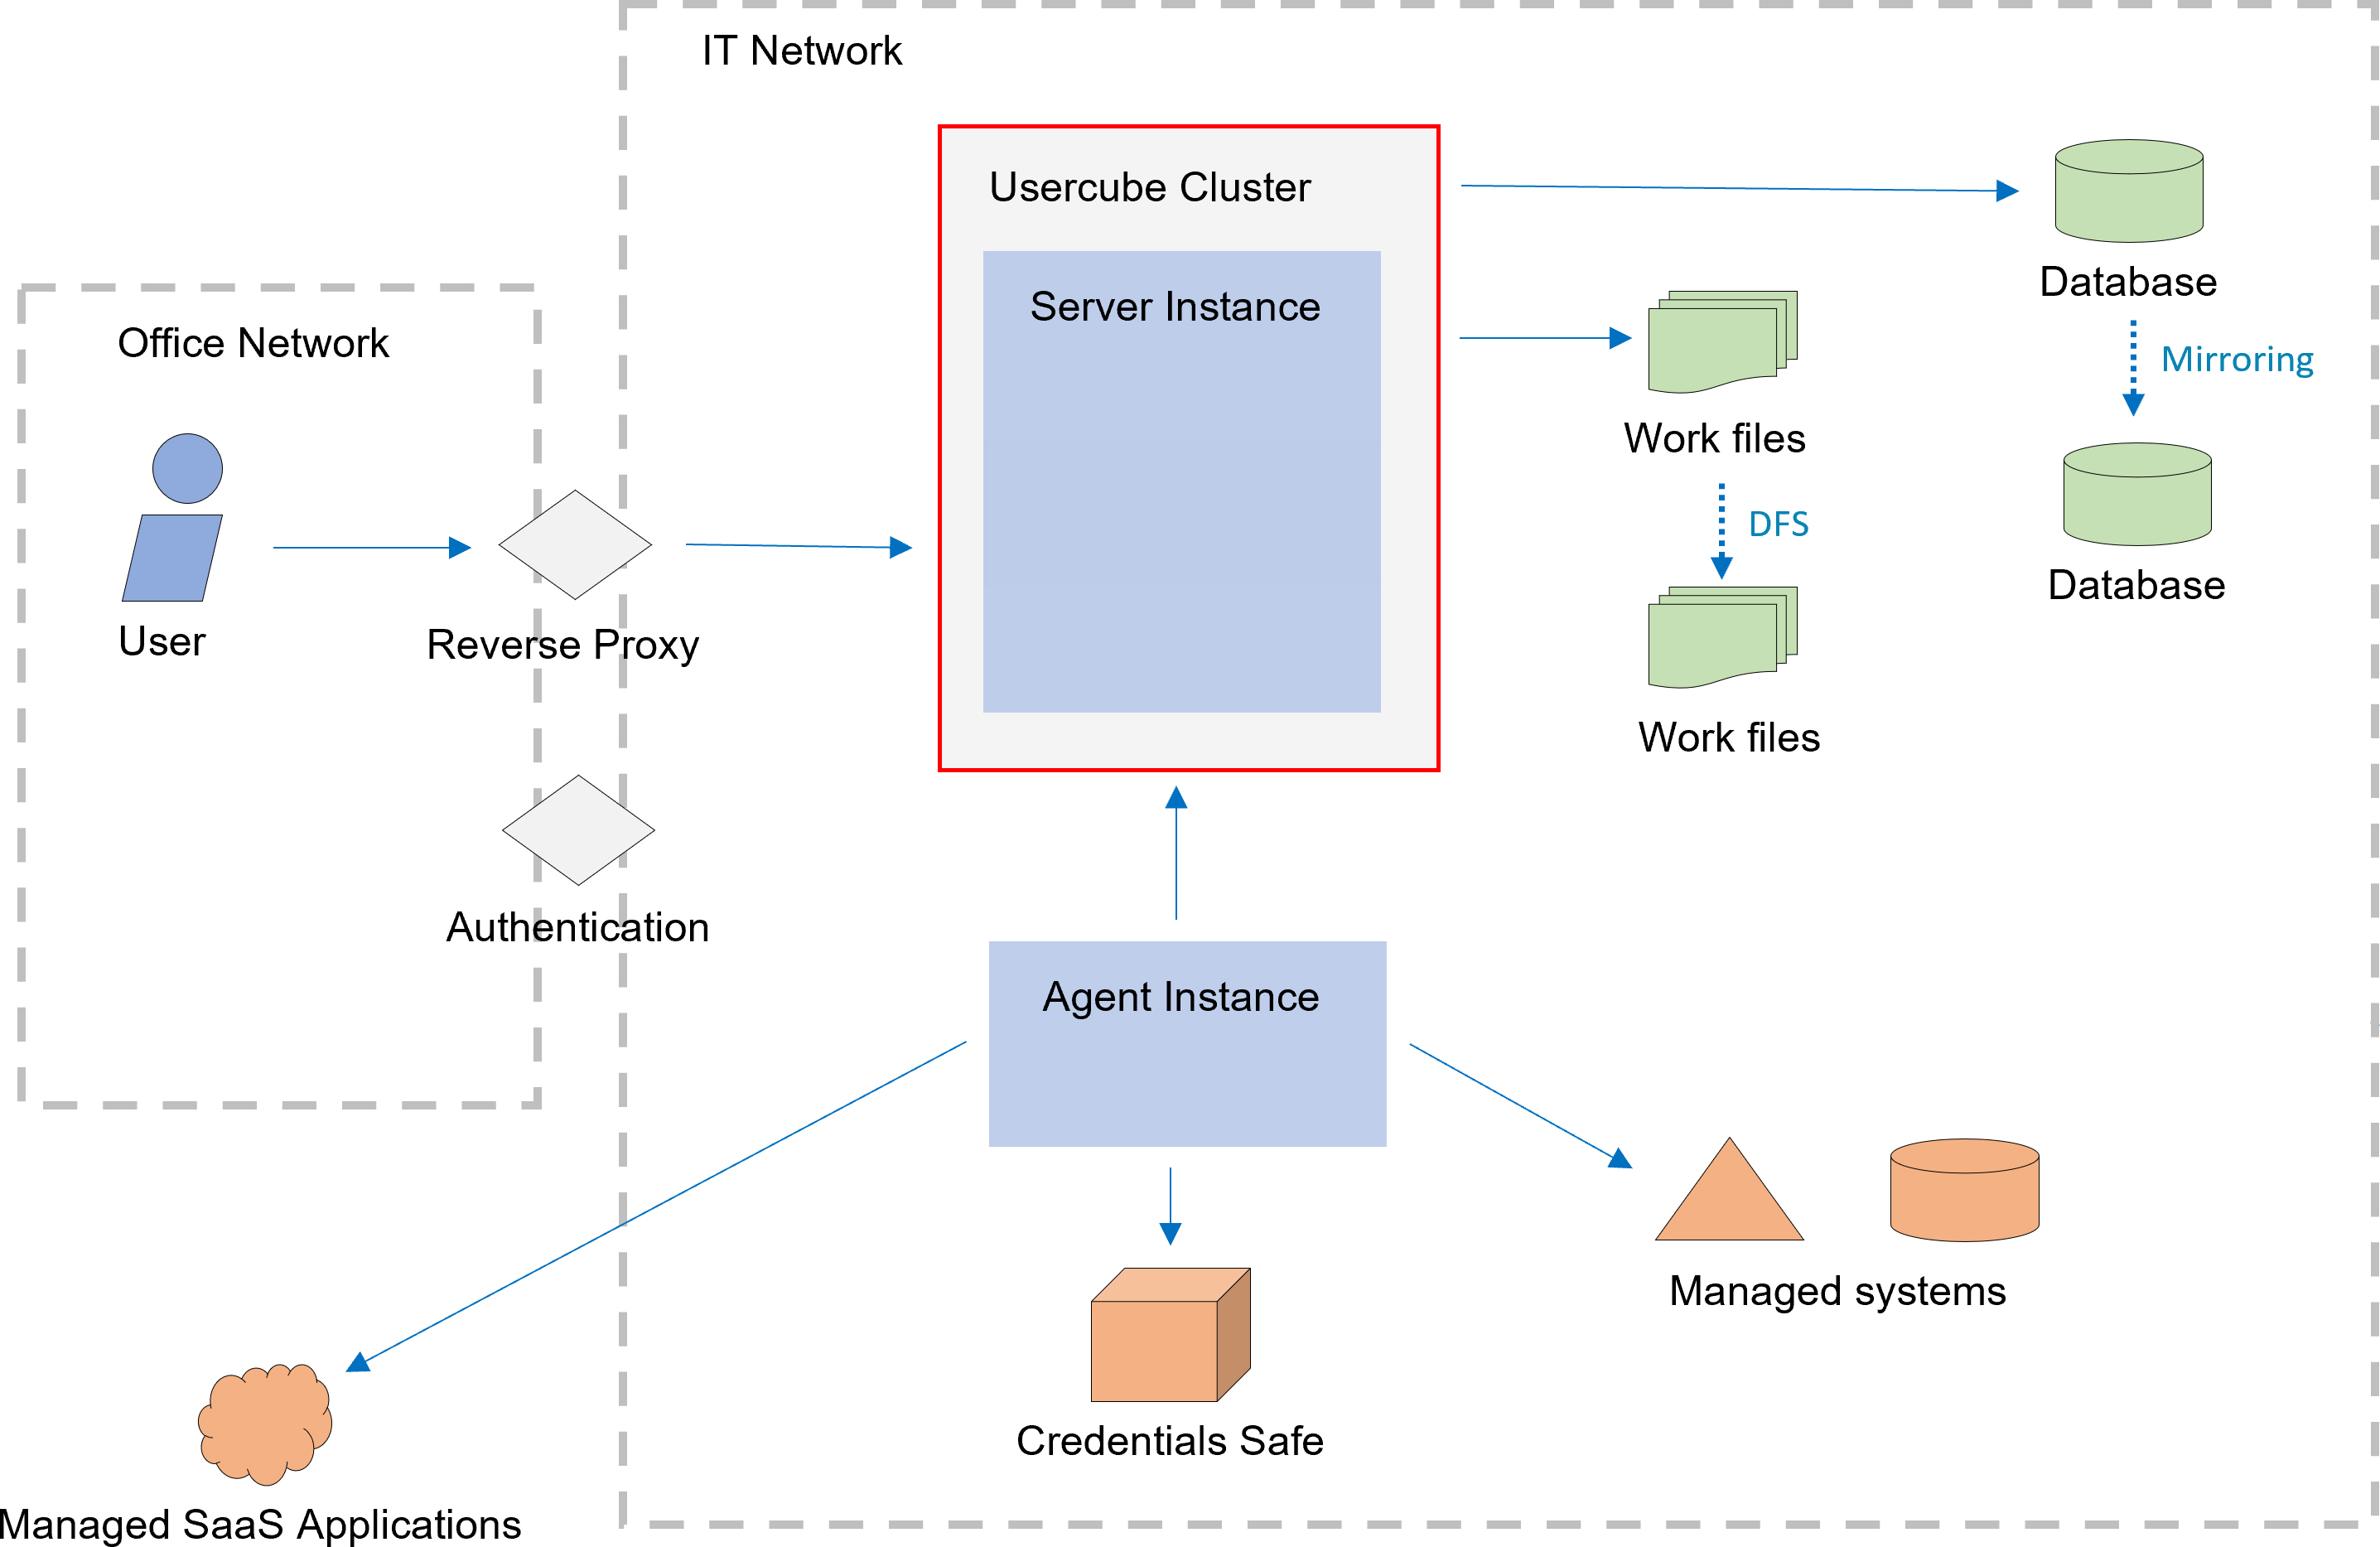
\includegraphics[width=5in]{Architecture_onPrem}
  \caption{Architecture on premises}
  \label{fig:Architecture_onPrem}
\end{figure}

\subsection{Configuration}

A Usercube configuration is a set of XML files edited according the Usercube schema. The recommendations part of this section explains how to set up an editing environment for the configuration.

Regardless of the editing space, the configuration persists in the Usercube database. It's this stored configuration that is used at runtime. The Deploy configuration tool is used to import a new version of the configuration (from the XML files set).

The Export configuration tool can be used to export the current configuration (to a XML files set). The Usercube project's integration cycle consists in developing a configuration by successive imports in a test instance.

The XML configuration schema shows some similarities with the database schema but they are not the same.

\begin{figure}[htbp]
  \centering
  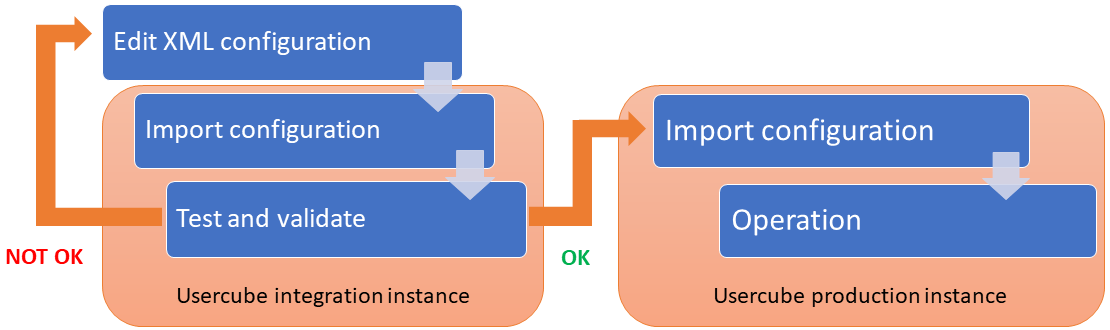
\includegraphics[width=5in]{configurationCycle}
  \caption{Usercube's configuration Cycle}
  \label{fig:configurationCycle}
\end{figure}

\subsection{Testing}


for testing we have different enviroments running in virtual machines. we deploy the new configuration to a testing instance and check if there is initial erros. Then the functional team is the one responsible to test the developments. After the test is done they send us back the ticket and then we save our code to build the next mep

\subsection{Deployment}


Deploy a local XML configuration by using the Deploy-Configuration executable and declaring at least: the configuration directory; the connection string of the database.
